% 原文PDF327の第9.5節見出しからPDF350末まで。
\subsectionlink{一般の振幅}\label{sec:9.5}

これで、一般の弦振幅の整合性を理解するために必要な要素が、すべてそろった。

モジュライ空間のグラフによる分解を与えたので、縫い合わせ形式によって、一般の弦振幅を図式的に表せる。まず、配管接合から得られる伝播関数を考えよう。モジュラス $q$ に対するゴースト挿入は
\begin{equation}
\oint\frac{dz}{2\pi i}\,b_{z_1z_1}
\left.\frac{\partial z_1}{\partial q}\right|_{z_2}
=\frac{b_0}{q}
\tag{9.5.1}\label{eq:9.5.1}
\end{equation}
であり、同様に $\bar q$ に対しては $\widetilde b_0/\bar q$ である。これらの挿入を含め、縫い合わせの表式 (9.4.6) を用いると、伝播関数に付随する因子は
\begin{equation}
\int_{|q|<1}\frac{d^2q}{q\bar q}\,
q^{\alpha'(k_i^2+m_i^2)/4}
\bar q^{\alpha'(k_i^2+\widetilde m_i^2)/4}
\mathcal G^{ij}b_0\widetilde b_0
=\frac{8\pi\delta_{m_i^2,\widetilde m_i^2}\mathcal G^{ij}b_0\widetilde b_0}
{\alpha'(k_i^2+m_i^2-i\epsilon)}
\tag{9.5.2}\label{eq:9.5.2}
\end{equation}
となる。$n$ 弦結合は、縫い合わせ構成の頂点に現れる曲面に頂点演算子を挿入することで与えられる。
\begin{equation}
g(i_1,\ldots,i_n)=\sum_g\int_{\mathcal V_{g,n}}d^mt\,
\left\langle\prod_{k=1}^{m}B_k
\prod_{l=1}^{n}\widehat{\mathcal V}_{i_l}\right\rangle_g.
\tag{9.5.3}\label{eq:9.5.3}
\end{equation}
ここで $m=6g+2n-6$ はモジュライの数である。結合 (9.5.3) と伝播関数 (9.5.2) から作られる Feynman グラフは、弦振幅全体を再現する。ラベル $i$ は、ここでも各弦の状態と運動量を表す。第9.1節の木振幅は、この構造を具体的に示している。

最初の問題は振幅の有限性である。低次のさまざまな例と同様に、発散はモジュライ空間の境界からしか生じないと主張する。モジュライが有限の値をとるとき、縫い合わせ公式は無限個の弦状態の和を与えるが、この和は収束する。究極的には、量子状態を完全系で展開しているだけだからである。実際には、収束が保証されるのはユニタリな CFT に限られるが、弦の CFT の非ユニタリな部分は、十分扱いやすい。$X^0$ の CFT はユニタリな CFT からの解析接続で定義され、ゴースト CFT は Faddeev--Popov 行列式を生成するだけなので、適切なゲージを選んでいれば有限である。境界は、今や各伝播関数の $q\to0$ 極限として明示されており、積分 (9.5.2) はこれまでに何度も出会ったものである。これは解析接続によって定義され、通常の場の理論の伝播関数を与える。したがって特異性は伝播関数の極だけであり、中間状態に質量殻上の粒子が生成されることを表す。特に、これらは短距離ではなく長距離の発散である。

もう一つの問題はユニタリティである。4点木振幅については、これをかなり詳しく調べた。一般の振幅を Feynman 図の形にしたので、組合せ論を詳しく展開する代わりに、図式展開のユニタリティに関する場の理論の標準的な結果を引用するだけにしよう。また、第9.1節の最後で示した、中間状態の和が物理的状態の和に帰着するという証明も、場の理論と同様に一般化される。

まとめると、弦理論の摂動的有限性とユニタリティに関わる問題は、十分理解されているように見える。再び注意しておくと、26個の平坦な方向を仮定したのではなく、$d$ 個の平坦な方向と、中心電荷 $26-d$ をもつ正ノルムのコンパクト CFT だけを仮定した。もちろん、ボソン弦の平坦時空の S 行列のユニタリティについての議論は、いくらか形式的である。平坦時空は理論の解ではないからである。まずタキオン不安定性があり、さらにループによって宇宙項が誘起される。

光円錐ゲージに基づく、弦理論の有限性とユニタリティへの別のアプローチも、広く発展してきた。このゲージは共変性を放棄するが、いくつかの利点がある。モジュライ空間をかなり明示的に記述でき、振幅を、光円錐時間 $x^+$ に関して局所的な Hamiltonian をもつ場の理論の形で表せる。その摂動論が共変な摂動論と等価であることを示すことによって、共変性も確立されている。

\subsubsectionlink*{弦の発散}

先へ進む前に、弦の発散が長距離の効果であるという点を、もう少し詳しく説明しよう。$n$ 個の頂点演算子を含む1ループ振幅を考え、図9.8(a)のように $\tau$ を固定したまま、$m$ 個の演算子が集まる極限を取る。弦のループはもちろん重力を含み、図9.8(a)は、相互作用頂点が時空内で集まると紫外発散を生じた、図1.1(c)の重力子ループを思わせる。この弦振幅にも確かに発散があるが、それは時空の短距離ではなく、長距離から来る。図9.8(b)は共形的に等価な描像であり、$m$ 個の頂点演算子は長い円筒によってトーラスの残りの部分につながっている。この円筒を切り開いて状態の完全系を挿入すると、通常の表式 (9.5.2) が得られ、$q\to0$ が頂点演算子の一致する極限に対応する。したがって特異性は、時空の長距離を伝播することによる通常の極だけである。ここでも共形不変性は、世界面上の短距離を時空の長距離へ変える。

\begin{figure}[tbp]
\centering
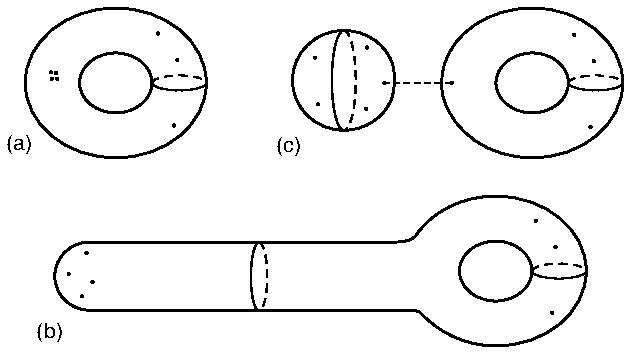
\includegraphics[width=0.82\linewidth]{figures/fig_9_8.pdf}
\caption{(a) $n$ 個の頂点演算子をもつトーラスで、そのうち $m$ 個が集まる極限。(b) 共形的に等価な描像。$m$ 個の頂点演算子は長い円筒の先端にある。(c) $m+1$ 個の頂点演算子をもつ球面と、$n-m+1$ 個をもつトーラスの積による縫い合わせ構成。}
\label{fig:9.8}
\end{figure}

$m=n$ と $m=n-1$ の場合には、特別な問題が生じる。$m=n$、すなわちすべての頂点演算子が集まる場合、運動量保存によって $k^\mu$ はゼロに強制される。質量のない状態では、その極は $1/0$ となり、通常の解析接続は役立たない。運動量保存により、振幅は質量のない極の真上に固定されるからである。これは第7.4節と同じタドポールであり、解決法も同じく背景場の補正である。ここでの発散は、一つの頂点演算子を含むトーラス振幅に比例する。

もう一つの問題となる場合、$m=n-1$ では、一つ、例えば $\mathcal V_n$ を除くすべての頂点演算子が集まる。運動量保存は、円筒を流れる運動量が $k^\mu=-k_n^\mu$ であることを要求する。しかし共形不変性は $k_n^2=-m_n^2$ を要求するので、$m_j^2=m_n^2$ の中間状態に対しては、中間運動量が極の真上に固定される。ここでも場の理論に同様の発散があり、図9.9に示した内部伝播関数は $1/0$ となる。この発散は、内部線 $j$ の質量が、質量殻上の外部粒子 $n$ の質量と同じときに必ず起こる。解釈は単純である。ループは粒子 $n$ の質量に対する輻射補正を表す。S 行列は、輻射補正を含めた\textbf{真の}質量殻上に外部運動量を取って定義され、その場合にはこの赤外発散は再びなくなる。ここで問題なのは、ループ内部の何らかの紫外発散ではなく、星印を付けた伝播関数の赤外発散であり、質量補正が有限であっても現れることに注意しよう。

\begin{figure}[tbp]
\centering
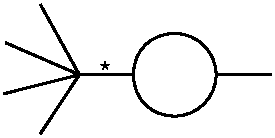
\includegraphics[width=0.57\linewidth]{figures/fig_9_9.pdf}
\caption{$m=n-1$ の場合に対応する場の理論のグラフ。運動学によって、星印を付けた伝播関数は発散する。ループによる有限の質量シフトと解釈される。}
\label{fig:9.9}
\end{figure}

弦の場合の解決法も同じである。頂点演算子に現れる運動量は、真の物理的質量に対応していなければならない。これは一般に、二乗が常に $1/\alpha'$ の整数倍だった、木レベルの質量とは同じでない。ある種の質量のない場、特にゲージボソンについては、ゲージ不変性が、あらゆる次数で質量がないままであることを保証する。なお、質量をもつ状態の質量シフトは通常複素数になる。これらの状態は、より軽い弦状態へ崩壊する不安定性をもつからである。

ここには一つ疑問がある。初めの方で、弦理論の整合性、すなわち世界面理論が共形不変であるという条件は、ベータ関数 (3.7.14) がゼロになることを要求すると見た。このベータ関数は高種数の曲面について何の情報も含まず、木レベルの弦の場の方程式に対応する。ループ補正を受けた背景のまわりで展開しようとすると、何が起きるのだろうか。実際には、すべてがちょうどうまく働く。図9.8の危険な極限は、発散だけでなく共形アノマリーも生む。これを直観的に見るために、その極限を図9.3(c)のように、球面に小さなハンドルを貼り付けたものとして描こう。小さなハンドルは局所演算子の級数で表せ、特に質量のないレベルからは
\begin{equation}
\partial X^\mu\bar\partial X_\mu\,\frac{dq\,d\bar q}{q\bar q}
\tag{9.5.4}\label{eq:9.5.4}
\end{equation}
がある。ここで、ハンドルの大きさが $a$ より大きいと要求して、座標不変な形で発散を切り落とす。すなわち、球面の計量が $dz\,d\bar z\,e^{2\omega}$ であるとき、$|q|e^\omega>a$ とする。積分 (9.5.4) の下限は
\begin{equation}
-4\pi\partial X^\mu\bar\partial X_\mu\ln(ae^{-\omega})
\tag{9.5.5}\label{eq:9.5.5}
\end{equation}
を与える。こうして計量の Weyl 因子への新たな依存性が生じ、これはシグマ模型の Weyl アノマリー $\beta_{\mu\nu}^G$、式 (3.7.14)、を補正する。Weyl 不変な理論を得るには、背景場が\textbf{弦のループ補正をすべて含めた} Weyl 不変性の条件、または等価に BRST 不変性の条件を満たさなければならない。シフトした背景からの Weyl アノマリーが、小さなハンドルからのものを打ち消す。これが \textbf{Fischler--Susskind 機構}である。図9.3(c)から、この発散と Weyl アノマリーは世界面の紫外効果と考えられる。ただし、通常の場の短波長の揺らぎによるものではなく、小さな位相幾何学的揺らぎによる。どのような種数でも、\textbf{固定した} Riemann 面上では局所的構造はトポロジーの影響を受けないことを強調しておく。発散と Weyl アノマリーを生むのは、Riemann 面についての積分である。

これは、伝播関数の相殺を用いた議論の破綻とみなすこともできる。運動学が振幅を極に固定するため、BRST 変分で生じうる表面項を除くのに解析接続を使えない。実際、その表面項は現れ、Weyl アノマリー (9.5.5) に対応する。ループ補正された背景では、背景のシフトによる BRST アノマリーが、モジュライ空間の境界によるものを打ち消す。弦特有の技術的な諸要素がすべてかみ合って、整合的な時空描像を与えるのである。

これを弦の摂動論で実行するのはかなり煩雑だが、幸い、必要になることはまれである。第一に、大部分の超対称理論では背景は補正されない。第二に、弦理論の長距離物理の解析は、普通は二段階で進めるのが最も効率的である。まず弦理論を用いて低エネルギー有効作用の形を導き、次に長距離では有効場の理論を用いる。そうすれば、弦の段階で赤外発散を扱う必要はない。今の場合、タドポールは有効作用中のポテンシャルエネルギー項
\begin{equation}
\delta\boldsymbol S=-\sum_\chi\Lambda_\chi
\int d^dx\,(-G)^{1/2}e^{-\chi\Phi}
\tag{9.5.6}\label{eq:9.5.6}
\end{equation}
を意味する。$\Lambda_\chi$ は Euler 数 $\chi$ からのタドポールであり、作用の $\Phi$ 依存性は $e^\Phi$ が弦結合であることから従う。重力子とディラトンそれぞれのタドポールは、いくらか手間をかければ弦振幅から取り出せる。

同じ考え方は、質量シフトによる頂点演算子の補正や、質量のない粒子を含む理論の排他的振幅に現れるものなど、他の赤外発散にも拡張される。弦理論は長距離で場の理論に帰着するので、これらの場の理論の発散は、対応する弦理論の振幅にも現れなければならない。繰り返し強調すると、場の理論の紫外発散は一般に、その理論の有効範囲の根本的な限界を意味するが、赤外発散は通常、それ以外は完全に整合的な理論に対して、単に誤った問いを立てていることを意味する。誤った背景、誤った質量、包括的断面積を問うべきところで排他的断面積を問うこと、などである。弦理論でのこのような発散も、まさに場の理論と同じように扱うべきである。

得られたことを振り返ろう。ボソン弦に特有の問題を除けば、S 行列は有限かつユニタリである。基本となる機構はモジュラー不変性であり、時空のゲージ不変性を損なわずに紫外発散を切り落とす。もちろん、平坦時空のまわりの弱結合摂動論で弦理論が意味をもつとわかっただけでは、とても十分とはいえない。摂動論を超えて理論が意味をもつことを知り、非摂動的補正を計算する何らかの手段が欲しい。また、短距離における時空の本性について、弦理論が何を示唆するかも知りたい。本章の残りでは、これらの方向でなされてきた試みのいくつかを簡単に述べる。

\subsectionlink{弦の場の理論}\label{sec:9.6}

弦理論でここまで採ってきた方法と、量子場の理論の定式化とを比較するのは興味深い。世界面の経路積分は粒子の経路の和に相当し、しばしば\textbf{第一量子化}の記述と呼ばれる。一方、量子場の理論では、時空の場についての経路積分、またはそれと等価な Hamiltonian 形式から出発する。代わりに、量子場の摂動論を第一量子化の形で展開することもできる。その場合には、$n$ 本の粒子の経路が終わる時空点として、相互作用頂点を明示的に導入する必要がある。弦理論では、この第二段階は必要ない。特別な点はなく、トポロジーについての和が相互作用を生む。しかし、得られるのは摂動展開だけであり、この展開に含まれない重要な現象もある。標準模型では、クォークの閉じ込めや、弱い相互作用による有限温度でのバリオン数の非保存がその例である。これらが摂動級数の再総和に含まれるといっても、有用な意味はないようであり、むしろ、より一般的な理論の定式化を必要とする。

前節では弦振幅を、無限成分の場の理論の摂動論に見える、伝播関数と頂点の形で表した。これを、無限個の時空場についての経路積分から導くことはできるだろうか。また、ゲージ不変性と一般座標不変性を拡張し、理論の形を決定する何らかの原理があるだろうか。これが\textbf{弦の場の理論}の主題である。ここでは、ごく少数の考え方、特にここまでのアプローチに近いものを概説するにとどめる。詳細は文献を参照してほしい。

弦の波動汎関数 $\Psi[X]$ を、場の演算子、または等価に経路積分の積分変数へ昇格させるべきだという推測から始めよう。いわゆる第二量子化である。$\Psi[X]$ は、弦が時空内に描く曲線 $X^\mu(\sigma)$ に依存し、大まかにいえば、その配置の弦を生成または消滅させる。しかし、もっと正確にする必要がある。例えば $\Psi$ には曲線の再パラメーター化に対する不変性を要求すべきだろうか。また、Polyakov 計量 $g_{ab}$ にも依存させるべきだろうか。Faddeev--Popov ゴーストを含めた BRST 不変な理論の形から始め、そこから第二量子化すると、はるかにうまく進むようである。交換関係から $b$ と $c$ は互いに共役であり、$\widetilde b$ と $\widetilde c$ も同様である。したがって、例えば $c,\widetilde c$ を座標として扱えば、波動汎関数は $\Psi[X,c,\widetilde c]$ となる。そして、そのようなすべての汎関数についての経路積分
\begin{equation}
\int[d\Psi]\exp(i\boldsymbol S[\Psi])
\tag{9.6.1}\label{eq:9.6.1}
\end{equation}
を考える。まず開弦について、一つの具体的なアプローチを述べよう。

どのような対称性原理が弦の作用を制限するだろうか。頂点演算子とヌル状態の研究から、任意の汎関数 $\Lambda$ に対する対称性
\begin{equation}
\delta\Psi=Q_{\mathrm B}\Lambda
\tag{9.6.2}\label{eq:9.6.2}
\end{equation}
を推測できる。この不変性をもつ極めて単純な作用がある。
\begin{equation}
\boldsymbol S_0=\frac12\langle\!\langle\Psi|Q_{\mathrm B}|\Psi\rangle.
\tag{9.6.3}\label{eq:9.6.3}
\end{equation}
運動方程式は単に
\begin{equation}
Q_{\mathrm B}\Psi=0
\tag{9.6.4}\label{eq:9.6.4}
\end{equation}
である。

これが妥当であることを見る一つの方法は、弦の各内部状態に一つずつ対応する、無限個の通常の場で弦の場 $\Psi$ を展開することである。内部モード、すなわち重心 $x^\mu$ 以外のすべてに対する波動関数の完全系を $\Psi_i[X',c,\widetilde c]$ としよう。一般の状態は
\begin{equation}
\Psi[X,c,\widetilde c]
=\sum_i\Phi_i(x)\Psi_i[X',c,\widetilde c]
\tag{9.6.5}\label{eq:9.6.5}
\end{equation}
と展開でき、展開係数は残りの変数 $x^\mu$ の関数となる。弦の場の経路積分は、成分関数に対する経路積分の無限積
\begin{equation}
\int[d\Psi]\longrightarrow\prod_i\int[d\Phi_i]
\tag{9.6.6}\label{eq:9.6.6}
\end{equation}
になる。いつものように、基底状態の汎関数 $\Psi_0$ から出発し、上昇演算子によって残りの状態を作れる。例えば、最初の二つのレベルのすべての状態を残すと、
\begin{equation}
\begin{split}
\Psi=\bigl[&
\varphi(x)+A_\mu(x)\alpha_{-1}^\mu+B(x)b_{-1}
+C(x)c_{-1}+\varphi'(x)c_0\\
&+A'_\mu(x)\alpha_{-1}^\mu c_0+B'(x)b_{-1}c_0
+C'(x)c_{-1}c_0+\cdots\bigr]\Psi_0.
\end{split}
\tag{9.6.7}\label{eq:9.6.7}
\end{equation}
ここで $\varphi$ はタキオン場、$A_\mu$ はゲージ場であり、$B,C$ は時空ゲージ対称性に付随する Faddeev--Popov ゴースト場である。プライムの付いた場はすべて、ゲージ変換で消せるか、補助場である。補助場とは、微分方程式ではなく代数方程式を満たし、消去できる場をいう。すると、対称性 (9.6.2) が $A_\mu$ の通常のゲージ変換を含み、作用が $\varphi$ に対して Klein--Gordon 形、$A_\mu$ に対して Maxwell 形であることを確かめられる。したがって BRST による弦の場の形式は、時空のゲージ不変性を非常に簡潔に一般化している。

\begin{figure}[tbp]
\centering
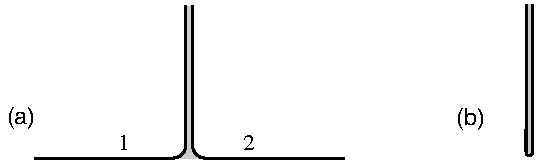
\includegraphics[width=0.74\linewidth]{figures/fig_9_10.pdf}
\caption{(a) $\Psi_1$ の右半分と $\Psi_2$ の左半分を畳み込む $\Psi_1*\Psi_2$。陰を付けた領域の経路積分として定義し、その幅をゼロにすると考えてよい。(b) $\Psi$ の右半分と左半分を畳み込む $\int\Psi$。}
\label{fig:9.10}
\end{figure}

相互作用も、かなりうまく構成できる。図9.10(a)に描いた汎関数積分によって、弦の場の積 $\Psi_1*\Psi_2$ を定義する。これは $\Psi_1$ の右半分と $\Psi_2$ の左半分の重なりを取る。また、図9.10(b)のように、単一の弦の波動汎関数の右半分と左半分の重なりを与える演算 $\int$ も定義する。相互作用する理論を作るため、ゲージ変換に非線形項を加える。
\begin{equation}
\delta\Psi=Q_{\mathrm B}\Lambda+g\Psi*\Lambda-g\Lambda*\Psi.
\tag{9.6.8}\label{eq:9.6.8}
\end{equation}
$*$ 積は結合的であり、積分路の議論により、$Q_{\mathrm B}$ は微分として
\begin{equation}
Q_{\mathrm B}(\Psi_1*\Psi_2)
=(Q_{\mathrm B}\Psi_1)*\Psi_2+\Psi_1*(Q_{\mathrm B}\Psi_2)
\tag{9.6.9}\label{eq:9.6.9}
\end{equation}
と作用することを示せる。これらから、対称性 (9.6.8) が閉じることが従う。巡回性
\begin{equation}
\int\Psi_1*\Psi_2=\int\Psi_2*\Psi_1
\tag{9.6.10}\label{eq:9.6.10}
\end{equation}
を用いると、不変な作用を
\begin{equation}
\boldsymbol S=\frac12\int\Psi*Q_{\mathrm B}\Psi
+\frac{2g}{3}\int\Psi*\Psi*\Psi
\tag{9.6.11}\label{eq:9.6.11}
\end{equation}
と書ける。$\Psi$ を、対応する頂点演算子 $\mathcal V_\Psi$ をもつ半円板に置き換えて、CFT によって書くのも有用である。
\begin{equation}
\boldsymbol S=\frac12
\langle\mathcal V_\Psi Q_{\mathrm B}\cdot\mathcal V_\Psi\rangle_{D_2}
+\frac{2g}{3}\langle
\mathcal V_\Psi\mathcal V_\Psi\mathcal V_\Psi\rangle_{D_2}.
\tag{9.6.12}\label{eq:9.6.12}
\end{equation}
頂点演算子の位置と共形座標枠は式 (9.6.12) に明示していないが、図9.11のとおりである。三つの頂点演算子の半円板を円板の中に収めるため、$z^{2/3}$ 写像を用いる。この作用は重要な確認を通過する。円板上の経路積分がゼロでないのは、挿入の全ゴースト数が $Q^{\mathrm g}=3$ の場合だけである。物理的状態の頂点演算子はすべてゴースト数1をもつので、作用 (9.6.12) の両項はゼロでない。作用 (9.6.11) は不変なので、ゲージ場に対して非 Abel な Yang--Mills 作用に帰着すると期待でき、実際にそうなる。

\begin{figure}[tbp]
\centering
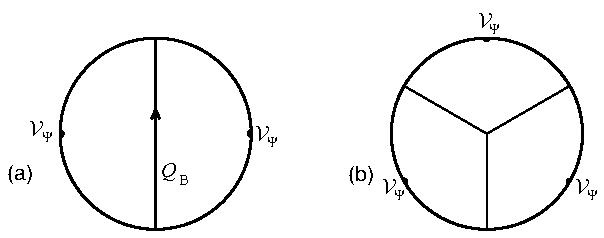
\includegraphics[width=0.78\linewidth]{figures/fig_9_11.pdf}
\caption{弦の場の作用の CFT 表現。(a) 運動項、(b) 相互作用。各頂点演算子を囲む通常の半円を扇形へ変えるため、$z^{2/3}$ の共形変換を用いる。}
\label{fig:9.11}
\end{figure}

Siegel ゲージは $b_0\Psi=0$ である。運動項の作用では、$Q_{\mathrm B}$ のうち $c_0L_0$ の項だけが残る。成分ごとに $L_0\propto p^2+m^2$ なので、これは電磁力学でおなじみの共変ゲージに相当する。伝播関数
\begin{equation}
\int_0^\infty dt\,\exp(-tL_0)=L_0^{-1}
\tag{9.6.13}\label{eq:9.6.13}
\end{equation}
は、任意の長さの帯についての積分にすぎない。頂点は図9.11(b)から扇形を取り除いたもので、三本の帯の端を「Y」字に結合する。これは Riemann 面の和として記述した開弦理論と等価であり、特にモジュライ空間を完全に一度だけ覆うことも示されている。一方で、これは驚くべきことではない。弦の場の理論には時空ゲージ不変性 (9.6.8) があるので、ヌル状態は S 行列から脱結合する。われわれは、ヌル状態の脱結合が弦振幅の形を決め、モジュライ空間を完全に覆う必要性も含むと論じた。そうでなければ、全微分項がヌル状態の結合を与えてしまう。他方で、モジュライ空間は複雑であり、明示的な記述はほとんど知られていない。この弦の場の理論が与える、Feynman グラフについての和と、各グラフの帯の長さについての積分による記述は、弦の場の理論による構成よりわずかに前に、数学者たちによって発見された。\footnote[2]{物理に動機付けられたモジュライ空間の別の記述は、光円錐ゲージから得られる。そこでのモジュライは、相互作用の時刻、中間状態の運動量 $p^+$、および各中間閉弦のツイスト角である。}

この場の理論の奇妙な特徴を指摘しておこう。弦の場の理論はモジュライ空間全体を覆うと述べたが、アニュラスから知っているように、そこには閉弦の極を生む極限が含まれる。明示的な閉弦場は存在しないにもかかわらず、そうなのである。閉弦の極は、帯の長さが無限大ではなくゼロになるところから現れる。\footnote[3]{このため、この形の弦の場の理論は、前節の目的には適さない。予想外の発散を除くため、頂点に短い管を付け加え、さらに、省かれたモジュライ空間の領域を覆うために、閉弦の伝播関数と頂点を加える必要がある。}
正確には、開弦の場の経路積分 (9.6.1) は、開弦と閉弦の両方を含む理論の振幅を生成する。ただし、境界をまったくもたず、開弦が結合できない曲面は生成されない。この点では、閉弦は、ある不明確な意味で開弦の「束縛状態」であるかのようである。

閉弦だけの理論では、閉弦の場を使って上の手順を繰り返せるが、いくらか複雑になる。自由作用 (9.6.3) の段階で、すでにゴースト数が合わない。物理的状態間の行列要素をゼロでなくするには、余分な $c$ ゴーストが一つ必要である。対処法は、弦の場 $\Psi$ とゲージ変換 $\Lambda$ が、$b_0-\widetilde b_0$ および $L_0-\widetilde L_0$ によって消されることを要求することである。すると作用
\begin{equation}
\boldsymbol S'_0=\frac12
\langle\!\langle\Psi|(c_0-\widetilde c_0)Q_{\mathrm B}|\Psi\rangle
\tag{9.6.14}\label{eq:9.6.14}
\end{equation}
は $\delta\Psi=Q_{\mathrm B}\Lambda$ のもとで不変になる。相互作用する理論へ進むと、$*$ に相当する結合的な積は存在せず、それに対応してモジュライ空間の単純な被覆もない。前節と同様に、モジュライ空間を覆うためには、場のより高い冪を含み、内部にハンドルももつ、高次の頂点 $\mathcal V_{g,n}$ を加えなければならない。得られる作用は、開弦の作用と同様に、\textbf{Batalin--Vilkovisky 形式}として知られるものを用いて、対称性原理から求められる。ゲージ固定すると、前節で述べた摂動論に至る。

時空ゲージ対称性から弦理論を導くことは、特に開弦の場合、非常に洗練されている。開弦の場の理論に閉弦も含まれることは興味深い。しかし、弦の場の理論が摂動論を超えて有用な道具となるかどうかは、まだ明らかではない。第14章で述べる、時空超対称性に基づく最近の非摂動的な進展には、役割を果たしていない。弦、あるいは弦の場は、「弦」理論の非摂動的定式化にとって、単に正しい自由度ではない可能性も十分ある。

\subsectionlink{高次での振る舞い}\label{sec:9.7}

弦の摂動論の高次での振る舞いについて、興味深い結果がある。場の理論から始めよう。積分
\begin{equation}
\int_{-\infty}^{\infty}dy\,
\exp\left[-\frac{y^2}{2!}-\lambda\frac{y^3}{3!}\right]
=\lambda^{-1}\int_{-\infty}^{\infty}dz\,
\exp\left[-\frac1{\lambda^2}
\left(\frac{z^2}{2!}+\frac{z^3}{3!}\right)\right]
\tag{9.7.1}\label{eq:9.7.1}
\end{equation}
を考える。ここで $z=y\lambda$ である。この積分は $\lambda\ne0$ で発散するが、ひとまずそれを無視し、$\lambda$ の冪に関する形式的展開として計算できる。
\begin{equation}
\sum_{n=0}^{\infty}\frac{(-\lambda)^n}{6^nn!}
\int_{-\infty}^{\infty}dy\,y^{3n}\exp(-y^2/2)
=(2\pi)^{1/2}\sum_{k=0}^{\infty}\lambda^{2k}C_{2k},
\tag{9.7.2}\label{eq:9.7.2}
\end{equation}
ただし
\begin{equation}
C_{2k}=\frac{2^k\Gamma(3k+1/2)}{\pi^{1/2}3^{2k}(2k)!}
\tag{9.7.3}\label{eq:9.7.3}
\end{equation}
である。この積分は、質量項と三次結合をもつスカラー場の理論の零次元極限である。$\lambda$ による展開は、伝播関数1、三次頂点 $-\lambda$ の Feynman グラフで表せる。すると定数 $C_{2k}$ は、三次頂点を $2k$ 個、または等価に $k+1$ 個のループをもつ真空グラフの総数を、適切な対称性因子で重み付けして数えているだけである。例えば、頂点が二つの真空グラフは二種類あり、それらの対称群の位数が8と12であることを読者は確かめられる。実際、$C_2=5/24=1/8+1/12$ である。高次での振る舞いを得るため、Stirling 近似 $n!\approx n^{n+1/2}e^{-n}$ を用いると、
\begin{equation}
C_{2k}\approx k^k\approx k!
\tag{9.7.4}\label{eq:9.7.4}
\end{equation}
となる。この近似は $k^a$ や $b^k$ の形の因子を除いて成り立つ。

四次項 $\lambda^2y^4/4!$ を加えてもよく、そうすると積分は収束する。$\lambda$ の冪は、$z$ に対する作用のすべての項が $\lambda^{-2}$ に比例するという要請で決まる。等価に、すべての $k+1$ ループ真空グラフが $\lambda^{2k}$ で重み付けされるということである。この追加項は結果を本質的には変えず、評価 (9.7.4) は述べた精度で依然として成り立つ。

場の理論を考えると、伝播関数と頂点はより複雑になる。しかし、高次での主要な振る舞いは通常、グラフの単純な数え上げから来る。異常な赤外または紫外の振る舞いがない限り、伝播関数と頂点は $b^k$ 程度の因子にしか寄与しない。級数は
\begin{equation}
\sum_{k=0}^{\infty}\lambda^{2k}k!f_{2k}
\tag{9.7.5}\label{eq:9.7.5}
\end{equation}
の形で、$f_{2k}\approx k^ab^k$ は $k!$ より緩やかに変化する。これは、$f_{2k}$ に予想外の相殺がない限り発散する。$\lambda$ が小さいと、各項はしばらく小さくなるが、やがて $k!$ が優勢になって増大する。和の最小項は
\begin{equation}
\exp[-O(1/\lambda^2)]
\tag{9.7.6}\label{eq:9.7.6}
\end{equation}
の程度である。したがってこれは、漸近級数としての摂動論の精度を示す。実際、インスタントンや動的な対称性の破れのように、摂動論のあらゆる次数でゼロになる効果は、典型的にこの程度である。例えば、級数 (9.7.2) の高次の振る舞いは、$z=-2$ にある、作用 $2/(3\lambda^2)$ の「インスタントン」、すなわち停留点に関係する。

弦理論では、モジュライ空間の Feynman グラフによる分解を用いて、同じ評価を確立できる。級数が (9.7.5) の形をもち、$f_{2k}$ が正で $b^k$ を下限にもつことが、明示的に示されている。したがって級数は発散し、Borel 総和すら可能ではない。Borel 総和では、級数 (9.7.5) を、より収束しやすい級数の Laplace 変換
\begin{equation}
\int_0^\infty dt\,\exp(-t)
\sum_{k=0}^{\infty}(t\lambda^2)^kf_{2k}
\tag{9.7.7}\label{eq:9.7.7}
\end{equation}
として書き直す。しかし $f_{2k}$ が正であることから、この新しい和は、収束するとしても正の $t$ 軸上に極をもち、積分は曖昧になる。したがって、弦理論には興味深い非摂動的現象があると期待すべきである。これは驚くべきことではない。低エネルギー極限だけでも、自明でない場の理論に帰着するからである。

閉弦理論に対する評価 (9.7.4) は下限であり、木レベルの三次頂点 $\mathcal V_{0,3}$ だけを残しても得られる。閉弦の頂点はあらゆる種数の Riemann 面から補正を受けるので、摂動論はさらに急速に増大するのではないかと考えられる。実際にそうなることを見る一つの方法は、開弦の場の理論が、少なくとも一つの境界をもつ、開弦と閉弦のあらゆる Riemann 面を含むことを思い出すことである。一つの境界をもつ曲面を、その境界が一点に縮んだ領域で考えよう。開弦のモジュライ空間のこの極限は、一つの頂点演算子をもつ閉曲面のモジュライ空間と等価である。この領域は、開弦のモジュライ空間全体に比べて著しく小さいわけではないと示せるので、同じ評価が成り立ち、摂動級数は
\begin{equation}
\sum_{k=0}^{\infty}g_{\mathrm o}^{2k}O(k!)
=\sum_{k=0}^{\infty}g_{\mathrm c}^{k}O(k!)
\tag{9.7.8}\label{eq:9.7.8}
\end{equation}
のようになる。

$g_{\mathrm c}^{2g}$ に比例する種数 $g$ の項は、$(2g)!$ 程度の係数をもつ。これは場の理論に特徴的な $g!$ より大きく、$\mathcal V_{0,3}$ だけから得た下限も $g!$ であった。明らかに、高次振幅の最大部分は頂点 $\mathcal V_{g,n}$ の内部に含まれ、モジュライ空間の内部から来る。したがって、
\begin{equation}
\exp[-O(1/g_{\mathrm c})]
\tag{9.7.9}\label{eq:9.7.9}
\end{equation}
程度の非摂動的効果が期待される。これは弱結合では、場の理論に特徴的な $\exp[-O(1/g_{\mathrm c}^2)]$ よりはるかに大きい。この高次での振る舞いは、第9.9節で述べるいくつかの簡単化された模型で初めて観察された。第13章で見るように、少なくともいくつかの超対称な弦理論では、これらの効果が D ブレーンと関係することが、今ではわかっている。

\subsectionlink{高エネルギーと高温}\label{sec:9.8}

弦の力学をよりよく理解するには、さまざまな極限での振る舞いを調べるとよいだろう。本節では、弦理論のいろいろな高エネルギー極限を考える。

\subsubsectionlink*{硬散乱}

Veneziano 振幅と Virasoro--Shapiro 振幅から Stirling 近似で求めた、硬散乱の振る舞いを再び考えよう。積分表示 (6.6.5) に戻る。
\begin{equation}
\frac{8\pi i g_{\mathrm c}^2}{\alpha'}
(2\pi)^{26}\delta^{26}\left(\sum_i k_i\right)
\int_{\mathbb C}d^2z_4\,
|z_4|^{-\alpha'u/2-4}|1-z_4|^{-\alpha't/2-4}.
\tag{9.8.1}\label{eq:9.8.1}
\end{equation}
$t/s$ を固定して $s\to\infty$ とする硬散乱領域では、指数は大きく、積分は指数の停留点に支配される。\footnote[4]{いつものように、積分は $z_4\to\infty$ で発散し、解析接続によって定義される。鞍点近似は、解析接続後の積分について正当化できる。}
$s,t,u\gg1$ の場合、鞍点は
\begin{equation}
\frac{\partial}{\partial z_4}
\left(u\ln|z_4|^2+t\ln|1-z_4|^2\right)
=\frac{u}{z_4}+\frac{t}{z_4-1}=0
\tag{9.8.2}\label{eq:9.8.2}
\end{equation}
で与えられ、解は $z_4=-u/s$ である。$s+t+u=O(1)$ を思い出そう。鞍点近似は、式 (6.6.13) のように、振幅
\begin{equation}
S\approx\exp[-\alpha'(s\ln s+t\ln t+u\ln u)/2]
\tag{9.8.3}\label{eq:9.8.3}
\end{equation}
を与える。

さらに一段階戻り、$z_4$ の積分から $X^\mu$ の経路積分を考えよう。これは鞍点
\begin{equation}
X_{\mathrm{cl}}^\mu(\sigma)
=i\sum_i k_i^\mu G'(\sigma,\sigma_i)
\tag{9.8.4}\label{eq:9.8.4}
\end{equation}
に支配される。$\sigma_i$ は頂点演算子の位置である。Green 関数が $\alpha'$ に比例することを思い出そう。高エネルギーでは、散乱領域の大きさはエネルギーに比例して増大し、$\delta X\approx\alpha'k$ となる。場の理論では、不確定性原理により、より高いエネルギーの硬散乱は、より短い距離 $\delta X\approx1/k$ を探る。弦理論では、弦スケールを超えるとそうならない。弦の摂動論では、このスケールより短い距離を探れないように見え、これが時空の限界距離だという考えにつながる。コンパクト化の実効的な下限 $R\approx\alpha'^{1/2}$ も、これを支持する。しかし第13章で見るように、非摂動的弦理論の最近の進歩は、さらに短い長さのスケールの存在を明らかにしている。

弦のループ展開の一般の次数では、振幅の主要な項は
\begin{equation}
\exp\left[-\sum_{i<j}k_i\cdot k_j\,G'(\sigma_i,\sigma_j)\right]
\tag{9.8.5}\label{eq:9.8.5}
\end{equation}
である。頂点演算子の位置と Riemann 面のモジュライの両方に関して、この指数の鞍点を求める必要がある。これは静電気の問題に似ている。指数は Riemann 面上の $n$ 個の点電荷 $k_i^\mu$ のエネルギーであり、$\mu$ は $d$ 個の異なる静電場を表し、$\mu=0$ ではエネルギーの符号が逆になる。運動量保存により背景電荷密度はゼロであり、$k_i^2$ は質量殻上の小さな値にとどまるので、繰り込み済みの自己エネルギーは無視できる。驚くべきことに、各種数において、おそらく主要な寄与を与える鞍点を求められる。Riemann 面
\begin{equation}
z_2^N=\frac{(z_1-a_1)(z_1-a_2)}{(z_1-a_3)(z_1-a_4)}
\tag{9.8.6}\label{eq:9.8.6}
\end{equation}
を考えよう。超幾何曲線 (9.2.9) と同様に、これは $S_2\times S_2$ の部分空間である。分岐切断で貼り合わされた $N$ 枚のシートとみなせ、種数は $N-1$ である。4点振幅について、電荷を分岐切断の位置 $a_i$ に置けば、振幅はその位置について停留する。その点では曲面は「垂直」で $\partial z_2/\partial z_1=\infty$ となり、対称性 $z_2\to\exp(2\pi i/N)z_2$ は勾配の垂直成分がゼロになることを要求するからである。残るのは位置 $a_i$ について極値化することだが、これは容易である。電場は、$N$ 枚のシートに分配される点を除いて、球面の $z=a_i$ に電荷を置いた場合と同じである。したがってエネルギーは、球面の場合の $N\cdot N^{-2}=N^{-1}$ 倍になる。三つの位置は Möbius 不変性によって、例えば $0,1,\infty$ に固定でき、第四の位置は球面と同じ条件 (9.8.2) で与えられる。ゆえに種数 $g$ では、
\begin{equation}
S_g\approx
\exp[-\alpha'(s\ln s+t\ln t+u\ln u)/2(g+1)]
\tag{9.8.7}\label{eq:9.8.7}
\end{equation}
となる。さらに計算すれば、鞍点のまわりの Gauss 型揺らぎを含められ、それが $S_g$ の係数を決める。$N$ 枚のシートからなる鞍点では、$X_{\mathrm{cl}}^\mu$ は単に $N=g+1$ で割られる。

この結果が妥当であることを確認する方法がある。小角領域 $-t/s\ll1$ では、
\begin{equation}
\exp[\alpha't\ln s/2(g+1)]
\tag{9.8.8}\label{eq:9.8.8}
\end{equation}
となる。$t^{1/2}$ は、入射粒子1から終状態の粒子3へ移される全運動量である。小角では、種数 $g$ の散乱過程を、$g+1$ 回の逐次的な散乱に分けられると考えられる。各散乱の重心エネルギー $s$ は同じであり、一方で $t_i$ には、全運動量移行が $t^{1/2}$ になるという制約がある。個々の散乱は $\exp(\alpha't_i\ln s/2)$ のように振る舞う。すると、各運動量移行を $t_i^{1/2}=t^{1/2}/(g+1)$ と等しくするのが最も効率的であり、振幅の積として結果 (9.8.8) が得られることを容易に確かめられる。これは、少数回の硬散乱で運動量を移すのが最も効率的な粒子散乱とは異なる。

弦の励起状態でも、頂点演算子の指数関数部分はタキオンの場合と同じである。したがって同じ鞍点が支配的となり、頂点演算子に $X_{\mathrm{cl}}^\mu$ を代入することになる。この同じ鞍点が、すべての状態、そして因子 $g+1$ を除けばすべての次数を支配するので、異なる状態の振幅の間には、あらゆる種数で成り立つ線形関係がある。したがって、厳密な振幅に対しても成り立つ可能性がある。量子場の理論では、高エネルギー散乱は、低エネルギーでは明らかでない対称性をしばしば明らかにする。ここで現れる関係も、そのような種類のものだと示唆されている。

級数 (9.8.7) を足し合わせることに、どの程度意味があるかは明らかでない。ここの結果を前節のものと比べるのは興味深い。いずれの場合も、境界付近で見いだされる場の理論的な振る舞いとは対照的に、興味深い物理を生むのはモジュライ空間の内部である。しかし高次の振る舞いは、モジュライ空間全体から来ており、特にその大きな体積に支配されていた。種数を固定した高エネルギーの振る舞いは、単一の点に支配される。

\subsubsectionlink*{Regge 散乱}

Regge 極限の解析も高次へ進められる。ここではそれは行わず、木レベルの Regge 物理の興味深い解釈を展開する。

Regge 散乱は、大部分の物理学者にとって硬散乱ほどなじみがない。これは、大きくブーストされた系を穏やかに探る方法である。系をブーストすると、時間の遅れによって内部過程が遅くなる。そのため、より高いエネルギーへ進むと、より多くの仮想的な自由度が見えると期待できる。

特に、一本の弦の量子揺らぎ、とりわけ基底状態の二乗平均平方根の大きさを考えよう。モード展開から、
\begin{equation}
\begin{split}
\langle0|[X^1(\sigma)-x^1]^2|0\rangle
&=\sum_{n=1}^{\infty}\frac{\alpha'}{2n^2}
\langle0|(\alpha_n\alpha_{-n}
+\widetilde\alpha_n\widetilde\alpha_{-n})|0\rangle\\
&=\alpha'\sum_{n=1}^{\infty}\frac1n
\end{split}
\tag{9.8.9}\label{eq:9.8.9}
\end{equation}
となる。これは発散するが、直接の物理的意味はない。時間スケール $\delta\tau$ の測定が感知できるのは、振動数が $\delta\tau^{-1}$ より小さいモードまでであり、本質的には $n\alpha'^{-1/2}<\delta\tau^{-1}$ である。対数発散は $\alpha'\ln(\alpha'^{1/2}/\delta\tau)$ になり、大きさはその平方根である。

この実効的な大きさの増大は、小さな $t$ での Regge 振幅 (6.6.12) に直接現れる。
\begin{equation}
s^{2+\alpha't/2}
\frac{\Gamma(-\alpha't/4-1)}{\Gamma(\alpha't/4+2)}
\sim\frac{s^2}{t}
\exp\left[-\frac{q^2\alpha'}2\ln(\alpha's)\right].
\tag{9.8.10}\label{eq:9.8.10}
\end{equation}
ここで $q^2=-t$ は運動量移行である。これは重力振幅 $s^2/t$ を形状因子で修正したものであり、その Fourier 変換は、大きさ $(\alpha'\ln\alpha's)^{1/2}$ の対象に対応する。一方の弦から見れば、他方の弦は $\alpha's$ 程度のブーストをもつので、その内部過程の時間分解能はこれに反比例し、先の大きさの評価と一致する。

対数の平方根は非常にゆっくり変化する関数であり、通常ならほとんど重要ではない。しかし、この振る舞いはブラックホール近傍の弦にとって非常に重要だと論じられてきた。第14章では、非常に大きくブーストされたときに弦がその真の姿を現すという考えを、別の観点から再び取り上げる。

\subsubsectionlink*{高温}

興味深い弦特有の振る舞いをもつ、同様の極限が高温である。大きなウェイト $h$ における分配関数の一般的な振る舞い (7.2.30) と、関係 $m^2=4(h-1)/\alpha'$ から、弦の状態密度 $n(m)$ は
\begin{equation}
\int_0^\infty dm\,n(m)\exp(-\alpha'\pi m^2\ell)
\approx\exp(4\pi/\ell)
\tag{9.8.11}\label{eq:9.8.11}
\end{equation}
を満たす。これは $n(m)\approx\exp(4\pi m\alpha'^{1/2})$ を意味する。したがって、一本の弦の熱分配関数は
\begin{equation}
\int_0^\infty dm\,\exp(4\pi m\alpha'^{1/2})\exp(-m/T)
\tag{9.8.12}\label{eq:9.8.12}
\end{equation}
となる。状態密度が指数関数的に増えるため、分配関数 (9.8.12) は、\textbf{Hagedorn 温度}
\begin{equation}
T_{\mathrm H}=\frac1{4\pi\alpha'^{1/2}}
\tag{9.8.13}\label{eq:9.8.13}
\end{equation}
より高い温度で発散する。Hagedorn 発散は次のように理解できる。長い弦のエネルギーは長さに比例する。エントロピーも示量的なので、やはり長さに比例する。低温ではエネルギーが支配的だが、高温ではエントロピーが支配的となり、任意に長い弦を作るのが有利になる。そのような弦の集団では密度が大きくなり、転移付近で相互作用が重要になる。

この発散は相転移を示唆する。実際、強い相互作用でも、高度に励起されたハドロンの状態密度は同様に増え、低温のハドロン相から高温のクォーク・グルーオン相への相転移がある。Hagedorn 発散が、基本弦にもクォーク・グルーオン構造に相当する何かを示しているのかを考えるのは興味深いが、明確な答えはない。

最後に、自由な弦の分配関数をもう少し詳しく論じよう。$d$ 次元における質量 $m$ の実スカラー場の自由エネルギー密度は
\begin{equation}
\begin{split}
F(T,m^2)
&=T\int\frac{d^{d-1}\boldsymbol k}{(2\pi)^{d-1}}
\ln[1-\exp(-\omega_k/T)]\\
&=-\int_0^\infty\frac{dt}{t}(2\pi t)^{-d/2}
\sum_{r=1}^{\infty}\exp\left(-\frac{m^2t}{2}
-\frac{r^2}{2T^2t}\right)
\end{split}
\tag{9.8.14}\label{eq:9.8.14}
\end{equation}
である。第二の形なら、弦のスペクトルについて容易に和を取れる。真空振幅 (7.3.12) と (7.3.6) の導出に従うと、26個の平坦な方向での自由エネルギー密度は
\begin{equation}
F(T)=-\int_R\frac{d\tau\,d\bar\tau}{2\tau_2}
(4\pi^2\alpha'\tau_2)^{-13}|\eta(\tau)|^{-48}
\sum_{r=1}^{\infty}
\exp\left(-\frac{r^2}{4\pi T^2\alpha'\tau_2}\right)
\tag{9.8.15}\label{eq:9.8.15}
\end{equation}
となる。積分は全領域
\begin{equation}
R:\qquad\tau_1\leq\frac12,\qquad|\tau_2|>0
\tag{9.8.16}\label{eq:9.8.16}
\end{equation}
にわたる。モジュラー不変な経路積分からの導出は演習9.7で与える。$\tau_2\to0$ では発散する可能性がある。被積分関数は $\tau$ の実部がゼロのとき最大なので、$\tau=i\tau_2$ と置こう。モジュラー変換 (7.2.44) から、この極限における eta 関数の漸近形は
\begin{equation}
\begin{split}
\eta(i\tau_2)&=\eta(i/\tau_2)\tau_2^{-1/2}\\
&\approx\exp(-\pi/12\tau_2)
\qquad(\tau_2\to0)
\end{split}
\tag{9.8.17}\label{eq:9.8.17}
\end{equation}
である。したがって $\tau$ 積分は $T<T_{\mathrm H}$ では収束し、$T>T_{\mathrm H}$ では発散する。

次の奇妙な観察がなされている。場の理論では、分配関数は時間の周期を $1/T$ にした Euclid 経路積分で与えられる。弦理論でも同じである（演習9.7）。すると T 双対性は高温と低温の振る舞いを関係付けるはずであり、実際、Hagedorn 温度は自己双対な温度の半分である。
\begin{equation}
\widetilde F(T)=F(T)+\rho_0
\tag{9.8.18}\label{eq:9.8.18}
\end{equation}
と定義する。これは自由エネルギーの熱的な部分 (9.8.15) と真空の部分 (7.3.6) の和である。経路積分の対数は $-\widetilde F(T)/T$ なので、T 双対性から
\begin{equation}
\frac1T\widetilde F(T)
=\frac{T}{4T_{\mathrm H}^2}
\widetilde F(4T_{\mathrm H}^2/T)
\tag{9.8.19}\label{eq:9.8.19}
\end{equation}
が従う。これは Hagedorn 温度より下の分配関数と、それより上の分配関数を関係付ける。$T>T_{\mathrm H}$ における Hagedorn 発散は、低温理論のタキオン発散を反映するものだが、タキオン発散のない超対称な弦でも、同様の形式的な結果が成り立つ。この関係を真剣に受け止めるなら、$T\to\infty$ において
\begin{equation}
\widetilde F(T)\longrightarrow\frac{T^2}{4T_{\mathrm H}^2}\rho_0
\tag{9.8.20}\label{eq:9.8.20}
\end{equation}
を得る。これが高エネルギーの自由度の数を測るものなら、その数は非常に少ない。$d$ 時空次元の単一の量子場は $T^d$ 程度の自由エネルギーをもつので、まるで弦理論の高エネルギー極限が\textbf{2時空次元}の場の理論のように見えることになる。これは Hagedorn 転移より下での、指数関数的に増大するスペクトルとはまったく異なり、相転移の本性への手がかりかもしれない。

\subsectionlink{低次元と非臨界弦}\label{sec:9.9}

場の理論は、時空の次元数を減らすと簡単になることが多く、そのような低次元理論は力学を理解するための有用な模型となってきた。弦理論でも同じことを試みたいが、弦理論には臨界次元の要請がある。コンパクト化はできるが、それでは自由度の数は減らない。弦はコンパクト方向にも依然として振動するからである。しかし、弦が実際に少ない次元を運動する、整合的な背景には、すでに出会っている。線形ディラトン背景 (3.7.18)、
\begin{align}
G_{\mu\nu}(x)&=\eta_{\mu\nu},\qquad
B_{\mu\nu}(x)=0,\qquad\Phi(x)=V_\mu x^\mu,
\tag{9.9.1a}\label{eq:9.9.1a}\\
V_\mu&=\delta_\mu{}^1\left(\frac{26-D}{6\alpha'}\right)^{1/2}
\tag{9.9.1b}\label{eq:9.9.1b}
\end{align}
がそれである。$D<26$ ではディラトンの勾配は空間的であり、ここでは1方向に取った。

実効的な弦結合 $e^\Phi$ は $x^1$ の関数で、大きな $x^1$ で発散する。このため弦の摂動論を用いるのは難しいが、幸い、摂動論が有効な、少し異なる背景がある。背景 (9.9.1) をタキオン作用 (6.6.16) に代入すると、線形化されたタキオンの場の方程式
\begin{equation}
-\partial^\mu\partial_\mu T(x)
+2V^\mu\partial_\mu T(x)-\frac4{\alpha'}T(x)=0
\tag{9.9.2}\label{eq:9.9.2}
\end{equation}
を得る。これは、線形ディラトンのエネルギー運動量テンソル (2.5.1) に対して、指数型頂点演算子が Weyl 不変となる条件である。解は
\begin{equation}
T(x)=\exp(q\cdot x),\qquad
(q-V)^2=\frac{2-D}{6\alpha'}
\tag{9.9.3}\label{eq:9.9.3}
\end{equation}
である。ディラトンと同様に $x^1$ だけに依存する解を探すと、
\begin{equation}
q_1=\alpha_\pm
=\left(\frac{26-D}{6\alpha'}\right)^{1/2}
\pm\left(\frac{2-D}{6\alpha'}\right)^{1/2}
\tag{9.9.4}\label{eq:9.9.4}
\end{equation}
となる。$D>2$ ではこれは複素数なので、タキオンは振動するが、$D\leq2$ では実指数関数が得られる。ただし臨界値 $D=2$ では、これに一次関数が掛かる。もちろん、タキオンの場の方程式には非線形補正がある。しかし、かなり微妙な理由により、解 $\alpha_-$ だけが特異性のない背景を与える点を除けば、これが背景の定性的な形を変えないことを示せる。

$D\leq2$ では、弦の基底状態を「タキオン」と呼ぶのは実は不適切である。この場は安定だからである（演習9.8）。また $D\leq2$ では、実指数関数 $T(x)=T_0\exp(\alpha_-x^1)$ が、結合の発散する、大きな正の $x^1$ の領域への伝播を妨げる。これを見るために、世界面作用
\begin{equation}
S_\sigma=\frac1{4\pi\alpha'}\int_M d^2\sigma\,g^{1/2}
\left[g^{ab}\eta_{\mu\nu}\partial_aX^\mu\partial_bX^\nu
+\alpha'RV_1X^1+T_0\exp(\alpha_-X^1)\right]
\tag{9.9.5}\label{eq:9.9.5}
\end{equation}
を考えよう。大きな $x^1$ では、指数関数的なタキオンが線形ディラトンに勝り、経路積分が抑制される。これは、タキオン背景による弦の有効ポテンシャルに対応する。物理的には、$x^1\to-\infty$ に、結合がゼロに近づく漸近領域がある。正の $x^1$ へ伝播する弦は互いに相互作用し、ポテンシャルで反射されて漸近領域へ戻る。実効結合の最大値は、エネルギーとポテンシャルの強さ $T_0$ によって決まる。図9.12に示すこの描像はいささか風変わりだが、可解模型を見つけるという目的からは、追究する価値がある。かなり似た物理をもつ模型である静的模型は、量子場の理論の本性を解き明かすうえで役割を果たした。

\begin{figure}[tbp]
\centering
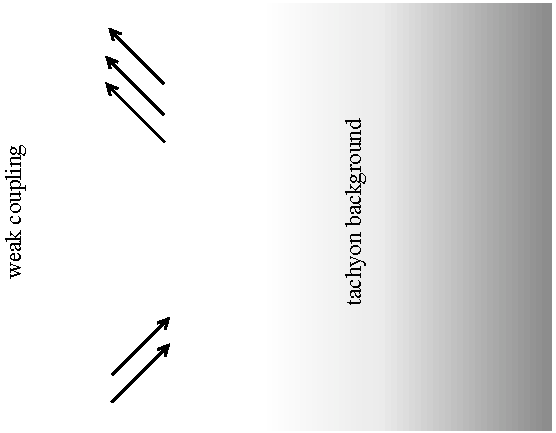
\includegraphics[width=0.73\linewidth]{figures/fig_9_12.pdf}
\caption{ディラトン背景とタキオン背景をもつ時空。相互作用の強さは右へ進むほど増えるが、タキオン背景からの有効ポテンシャルによって遮られる。}
\label{fig:9.12}
\end{figure}

$D>2$ では、タキオン背景の物理的な効果はそれほど明らかでないが、この場合にも障壁として働くと論じられてきた。しかし、別の理由から $D\leq2$ が中心に研究されてきた。これらの理論は、実際に解けるのである。まず、弦を量子化すると、ゲージ対称性が二組の振動子を取り除くので、$D\leq2$ では何も残らないことに注目しよう。残るのは重心運動、すなわち単一のスカラーだけである。\footnote[5]{特別な運動量では、追加の物理的状態が見いだされる。これらは弦の場の理論の破れていない対称性と解釈でき、おそらく理論の可解性に役割を果たしている。}
それでも、弦理論を直接解くのはなおかなり難しい。まず、作用 (9.9.5) をもつ世界面の経路積分を評価しなければならない。指数関数的なタキオン場のため、これはもはや自由理論ではない。これは \textbf{Liouville 場の理論}として知られる。古典的には可積分であり、大きな努力によっていくつかの量子振幅も求められている。しかし弦理論を解くには、さらに各種数で得られた結果を、Riemann 面のモジュライ空間にわたって積分する必要がある。この空間が複雑であることは、すでに見た。驚くべきことに、まったく異なる方法によって、あらゆる次数の完全な振幅が求められている。これを説明するには、まず別の考えを導入しなければならない。

\subsubsectionlink*{非臨界弦}

$d$ 次元 Euclid 空間内の2次元曲面についての和で定義される、統計力学系を考えよう。さらに曲面には、長さの尺度と解釈できる何らかの内部自由度があるとする。系を記述する自然な場は、埋め込み $X^\mu(\sigma)$ と計量 $g_{ab}(\sigma)$ である。しかし、長さが問題から消える、すなわち理論が Weyl 不変になる特別な理由はない。そのため、これは\textbf{非臨界弦}と呼ばれる。この系の最も低い次元の作用、あるいは統計力学の文脈で経路積分を考えているので Boltzmann の重みは、Polyakov 作用に、世界面の宇宙項を加えたものとなる。臨界弦では、この項は Weyl 不変性によって禁じられる。
\begin{equation}
S=\frac1{4\pi\alpha'}\int_M d^2\sigma\,g^{1/2}
\left(g^{ab}\partial_aX^\mu\partial_bX_\mu+\mu\right).
\tag{9.9.6}\label{eq:9.9.6}
\end{equation}

Weyl 不変性がなくても、微分同相不変性を用いて計量を部分的に固定できるが、一つの自由度が残る。
\begin{equation}
g_{ab}(\sigma)=\exp(2\phi(\sigma))\widehat g_{ab}(\sigma).
\tag{9.9.7}\label{eq:9.9.7}
\end{equation}
$\widehat g_{ab}$ はゲージの選択であり、計量のスケール $\phi$ は依然として経路積分される。このゲージ固定の Faddeev--Popov 行列式は、式 (3.4.19) と同じである。後者における Weyl ゲージ固定の寄与は自明だからである。曲率が
\begin{equation}
g^{1/2}R=\widehat g^{1/2}
\left(\widehat R-2\widehat\nabla^2\phi\right)
\tag{9.9.8}\label{eq:9.9.8}
\end{equation}
となる計量 (9.9.7) を代入し、場に依存しない項を省くと、作用と Faddeev--Popov 行列式を合わせたものは
\begin{equation}
\begin{split}
S=\frac1{4\pi\alpha'}\int_M d^2\sigma\,\widehat g^{1/2}
\biggl[&
\widehat g^{ab}\partial_aX^\mu\partial_bX_\mu+\mu\exp2\phi\\
&+\frac{13\alpha'}3
\left(\widehat g^{ab}\partial_a\phi\partial_b\phi+\widehat R\phi\right)
\biggr]
\end{split}
\tag{9.9.9}\label{eq:9.9.9}
\end{equation}
となる。Faddeev--Popov 行列式が $\phi$ の運動項を与えたことに注意しよう。これをディラトン・タキオン作用 (9.9.5) と比べると、著しく似ている。$d=D-1$ とし、新しい場 $\phi$ を $x^1$ と解釈し、作用 (9.9.5) では完全にゲージ固定できるので $g_{ab}\to\widehat g_{ab}$ と名前を変えると、同じ項がすべて現れる。いくつかの係数は少し異なり、すべてを一致させる $\phi$ のスケール変換は存在しない。それでも、実際にはこれらは同じ場の理論であると主張する。要点は、臨界弦の経路積分 (9.9.5) は $\widehat g_{ab}$ を計量として定義され、非臨界弦 (9.9.9) は $\exp(2\phi)\widehat g_{ab}$ を用いて定義されることである。測度の Weyl 変換を注意深く扱えば、一方から他方へ変換される。非臨界弦の定義には完全な計量 (9.9.7) だけが現れるので、
\begin{align}
\widehat g_{ab}(\sigma)&\longrightarrow
\exp(2\omega(\sigma))\widehat g_{ab}(\sigma),
\tag{9.9.10a}\label{eq:9.9.10a}\\
\phi(\sigma)&\longrightarrow\phi(\sigma)-\omega(\sigma)
\tag{9.9.10b}\label{eq:9.9.10b}
\end{align}
によって何も変わりえないことに注目すれば、これは容易に理解できる。こうして非臨界弦は Weyl 不変性を獲得し、それだけで自由パラメーター $\mu$ を除くさまざまな係数が決まる。

Weyl 不変な理論と不変でない理論が等価になれるのは、奇妙に思えるかもしれない。要点は、場の理論では、ゲージ固定だけに使う余分な場も加えれば、余分な「見かけだけの」ゲージ対称性をいつでも加えられることである。結局、ゲージ対称性は記述の冗長性にすぎず、いつでも、より冗長な記述を採用できる。対称性 (9.9.10) では、Weyl 対称性と場 $\phi$ を単に相殺できるのは明らかである。しかし一般の弦背景、例えば埋め込み座標が Weyl 不変な平坦空間では、これは不可能であり、Weyl 不変性は「本物」である。

いずれにせよ、いよいよ要点に近づいた。非臨界弦は、三角形分割された曲面についての和で近似でき、二点の間の辺の数を長さの尺度とする。これらの三角形分割された曲面は大きな Feynman 図に似ており、実際、これを図式展開としてもつ量子系、すなわち\textbf{行列模型}が見つかる。行列模型の場は $N\times N$ 行列である。$N\to\infty$ とし、他の結合を調整すると、少なくとも $D\leq2$ では、大きく滑らかな曲面が支配的な臨界点があり、非臨界弦が回復される。さらに、行列模型は、やはり $D\leq2$ で、行列を対角化することで解ける。最終的に得られるのは、固有値の空間を運動する相互作用しないフェルミオンという、かなり単純な系である。そして上の手順をたどり直せば、すべての種数の弦振幅を計算できる。

これらの方法は本書の他の部分から大きく離れるので、詳細は参考文献に委ねなければならない。いずれにせよ、$D>2$ や超対称理論では、まだ有用なものにはなっていない。ただし第14章で見るように、多少異なる大 $N$ 行列の理論が、非摂動的弦理論として最近提案された。しかし、これらの模型から得られた重要な教訓を、少なくとも一つは挙げておくべきだろう。それは摂動論の $(2g)!$ の振る舞いである。これは、行列模型の明示的な解で初めて見られ、その後すべての弦理論で成り立つと論じられた。行列模型では、対応する $\exp[O(-1/g_{\mathrm c})]$ の効果は、固有値の空間でのフェルミオンのトンネル効果に関係する。これが、より高次元の弦理論の $\exp[O(-1/g_{\mathrm c})]$ の効果と関係付けられるかどうかは明らかでない。

\subsectionlink*{演習問題}
\addcontentsline{toc}{subsection}{演習問題}

\subsubsectionlink*{演習9.1}\label{ex:9.1}
(a) 共形変換を用いて、OPE (9.1.2) と期待値 (9.1.3) から内積 (9.1.29) が従うことを示せ。

(b) 基底 $|\widehat{\mathcal V}_j(k)\rangle$ で行列要素を取り、式 (9.1.28) の第二の等号を確認せよ。

\subsubsectionlink*{演習9.2}\label{ex:9.2}
(a) 球面に対する式 (9.1.17) と同様に、ただし今度はトレースを含む形で、トーラス上の4点振幅を演算子形式で書け。

(b) 頂点演算子の一つがヌル、すなわち $\widehat{\mathcal V}_1=\{Q_{\mathrm B},\mathcal X\}$ なら、トレースが、頂点演算子の位置に関する全微分と、$\tau,\bar\tau$ に関する全微分の和に等しいことを示せ。

\subsubsectionlink*{演習9.3}\label{ex:9.3}
(a) 四つの頂点演算子をもつトーラスに対し、前問 (a) の結果を用い、$w_1,w_2,w_3-w_4$ を固定し、$w_3$ と $2\pi\tau-w_3$ が $i\infty$ に近づく極限でのユニタリティを調べよ。これは二つのハンドルが退化する極限であり、ユニタリティはその振幅を、二つの木レベル4点振幅の積に関係付ける。

(b) 特に、全 Hilbert 空間 $\widehat{\mathcal H}$ にわたる和と、物理的 Hilbert 空間にわたる和が等しいという証明を繰り返せ。そのためには、異なるゴースト数をもつ中間状態の間の相殺が必要なことを示せ。この相殺は、ゲージ理論での Faddeev--Popov ゴーストと縦偏極ゲージボソンの相殺を、弦へ一般化したものである。

\subsubsectionlink*{演習9.4}\label{ex:9.4}
図9.6(a)の Feynman グラフが覆う領域についての、式 (9.3.7) の主張を確認し、このグラフが覆う他の二つの領域を求めよ。

\subsubsectionlink*{演習9.5}\label{ex:9.5}
(a) 弦の場の展開の項 (9.6.7) について、ゲージ変換 (9.6.2) と作用 (9.6.3) を明示的に書き下せ。

(b) 補助場と、ゲージ変換で完全に取り除ける場を消去し、得られる $A_\mu$ のゲージ変換と作用が期待される形をもつことを示せ。

\subsubsectionlink*{演習9.6}\label{ex:9.6}
$f_{2k}=k^ab^k$ に対し、級数 (9.7.5) の最小項が $\exp(-C/g^2)$ の程度であることを示せ。$C$ を求めるのに十分な精度で計算せよ。級数 (9.7.2) について、インスタントン作用と比較せよ。

\subsubsectionlink*{演習9.7}\label{ex:9.7}
量子論では、Euclid 時間の周期が $T^{-1}$ の Euclid 経路積分は、熱分配関数 $\exp[-\widetilde F(T)/T]$ を与える。弦の経路積分について、これが結果 (9.8.15) と一致することを示せ。唯一の微妙な点は、積分領域と巻き付き数についての和との関係である。（参考文献：McClain \& Roth (1987)\cite{McClain:1986id}。）

\subsubsectionlink*{演習9.8}\label{ex:9.8}
線形ディラトン背景 (9.9.1) におけるタキオンの波動方程式 (9.9.2) に対し、$D\leq2$ なら、任意の\textbf{有限エネルギー}の初期配置が、安定な、すなわち振動的な時間発展をすることを示せ。

\subsubsectionlink*{演習9.9}\label{ex:9.9}
$D=2$ の線形ディラトン背景における閉弦の重力子レベルについて、物理的状態条件を OCQ または BRST の形式で調べよ。運動量には複素数値を許せ。一般の運動量では物理的スペクトルは自明だが、二つの運動量では非自明な物理的状態があるはずである。

\subsubsectionlink*{演習9.10}\label{ex:9.10}
式 (9.8.14) を導け。ヒント：第二行で、$m^2$ が $m^2+\boldsymbol k^2$ になるように $\boldsymbol k$ の積分を導入する。次に $t$ を積分する。結果は初等関数で表される。最後に、$r$ の和は第一行の対数の級数展開である。
